\section{Procedure}
The experiment can be divided into two parts: first, the examination of various 
amplitude gratings, and second, the measurement of a phase modulating grating, 
thus the introduction into acousto-optics. The single steps are the following:
\begin{enumerate}
    \item
        Calibration and establishing the relationship between difference in time 
        read off the oscilloscope and distance between the corresponding maxima, 
        using a gauge grating with lattice constant $K_\mathrm{gauge} = 0.1 \,$mm.
    \item
        Examination of amplitude gratings, consisting of the following steps:
        \begin{enumerate}
            \item
                Measuring a sine amplitude grating and determining the distance of the first 
                order maximum. The laser beam is not widened and collimated, but 
                passes through the grating directly and is then projected onto a screen. 
            \item
                Determination of lattice constant and resolution of five amplitude gratings.
            \item
                Calculation of aperture function and further 
                determination of the ratio of slit width and grating constant of the first grating. 
        \end{enumerate}
        \item
            Examination of the phase grating induced by an ultrasonic wave. 
            This part consists of the following tasks:
        \begin{enumerate}
            \item
                Measuring the intensity distribution for different voltages applied to the cell;
            \item
                Comparing the results to Raman-Naht theory by fitting Bessel function on the 
                intensities of $m$th order;
            \item
                Determination of wave length of the ultrasonic wave.
        \end{enumerate}
\end{enumerate}

\section{Experimental setup}
The setup of the entire experiment is contained in one beam path. 
For the different parts of the experiment, the gratings or the tank 
filled with isooctane (referred to as the "ultrasonic cell") will be 
taken out or installed as necessary. An overview is given in figure \ref{fig:setup}.
Apart from the almost self explanatory part with lenses for widening and 
collimating the beam (for a higher resolution, see theory section \ref{sec:resolution}), 
as well as a third lens to project the beam in the Frauenhofer limit 
onto a single point at diode 1, 
there is one special feature: Instead of projecting the beam onto a screen and 
measuring the distances of the peaks directly, we use a rotating mirror which 
projects only a certain solid angle of the entire intensity distribution onto 
the opening of the diode 1. The constant rotational speed and existing gauge gratings 
can then be used establish a linear relationship between the signal recorded by the 
oscilloscope and the actual distance. A second beam, which is created by a beam splitter and 
takes a separate path, is used exclusively as a trigger signal for the oscilloscope.

\begin{figure}
    \centering
    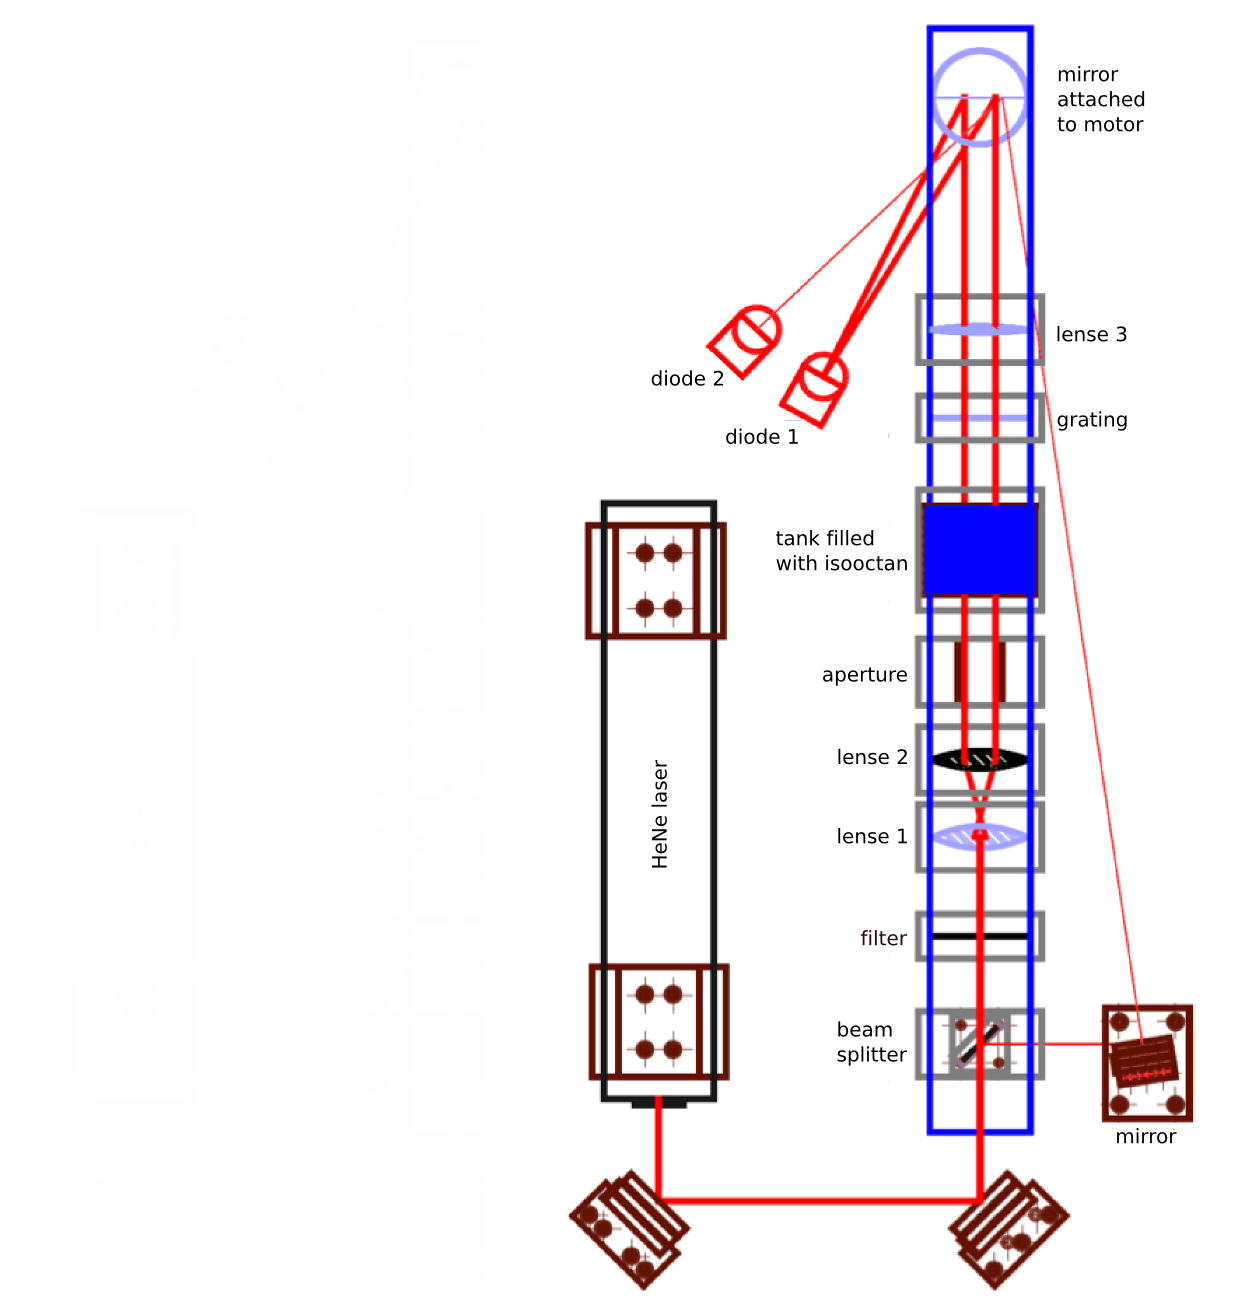
\includegraphics[width=1.0\textwidth]{figures/setup_bitmap.png}
    \caption{
        Scheme of the experimental setup. The tank or the gratings will be taken out 
        according to each part of the experiment.
        Modified, from \cite{ver}.
        }
    \label{fig:setup}
\end{figure}

